\documentclass[defaultstyle,10pt,master,Helvetica]{01.thesis}
% Helvetica is a similar font to Arial, with small differences.

%% Packages
\typeout{}
\typeout{--------------------------------------------------------------}
\typeout{ +---+ Thesis Template                            }
\typeout{ +---+      Version 2.0, August 2011                         }
\typeout{ +---+  for Instituto Superior Tecnico (IST),                 }
\typeout{ +---+  Universidade Técnica de Lisboa                         }
\typeout{ * Using Thesis Style form Pedro Tomás                                }
\typeout{ * Created to write Dissertations                             }
\typeout{ * Conforms with IST Master Degree format and with most important packages setup        }
\typeout{ * Should conform with IST PhD Degree format (not verified)   }
\typeout{                                                              }
\typeout{ AUTHOR: Miguel Amador and João Marques                                          }
\typeout{                                                              }
\typeout{Important: Use all files in the archive, since this is based in all them. Modify dummy files at wish.                                                              }
\typeout{--------------------------------------------------------------}
\typeout{}

% Defines an additional alphabet... not required in most cases
% ------------------------------------------------------------
% \DeclareMathAlphabet{\mathpzc}{OT1}{pzc}{m}{it}

% PACKAGE babel:
% ---------------
% The 'babel' package may correct some hyphenisation issues of latex.
% However in most situations it is not required.
\usepackage[english]{babel}

% PACKAGE fontenc:
% -----------------
% chooses T1-fonts and allows correct automatic hyphenation.
%\usepackage[T1]{fontenc}
\usepackage[latin1]{inputenc}

% Package ulem.
\usepackage{ulem} % Allows the use of other text emphatizer commands
\normalem %defines \emph{} to italic, instead of underline.
\raggedbottom %declaration makes all pages the height of the text on that page. No extra vertical space is added. The \flushbottom declaration makes all text pages the same height, adding extra vertical space when necessary to fill out the page.

% PACKAGE date time:
% -----------------
% Lets you alter the format of the date that \today returns.
\usepackage{datetime}
\newdateformat{todaythesis}{\monthname[\THEMONTH]  \THEYEAR}

% PACKAGE latexsym:
% -----------------
% Defines additional latex symbols. May be required for thesis with many math symbols.
\usepackage{latexsym}

% PACKAGE amsmath, amsthm, amssymb, amsfonts:
% -------------------------------------------
% This package is typically required. Among many other things it adds the possibility
% to put symbols in bold by using \boldsymbol (not \mathbf); defines additional
% fonts and symbols; adds the \eqref command for citing equations. I prefer the style
% "(x.xx)" for referering to an equation than to use "equation x.xx".
\usepackage{amsmath, amsthm, amssymb, amsfonts, amsbsy}

% PACKAGE multirow, colortbl, longtable:
% ---------------------------------------
% These packages are most usefull for advanced tables. The first allows to join rows
% throuhg the command \multirow which works similarly with the command \multicolumn
% The second package allows to color the table (both foreground and background)
% The third package is only required when tables extend beyond the length of one page;
% with compatibilities with the tabular environment. The last allow the definitions of landscape pages, allowing the use of a different orientation for wider graphics or tables. See package documentation to see the implementation.
\usepackage{multirow}
\usepackage{colortbl}
\usepackage{supertabular}
\usepackage{pdflscape}
% \usepackage{longtable}

% PACKAGE graphics, epsfig, subfigure, caption:
% ---------------------------------------------
% Packages for figures... well you will certainly need these packages, with the exception
% of the 'caption' package. This only allows to define extra caption options.
% Notice that subfigure allows to place figures within figures with its own caption. It
% should be avoided to create an eps file with subfigures. That will mean that you won't be
% able to reference those subfigures. Instead create an EPS file (the only graphics format supported
% by latex) for each of the subfigures and then use the command \subfigure (see below).
\usepackage{graphics}
\usepackage{graphicx}
\usepackage[caption=false]{subfig}
%\usepackage[footnotesize,bf,center]{caption}
\usepackage{dcolumn}
\usepackage{bm}
\usepackage{booktabs}
\usepackage{rotating}
\usepackage{multirow}

%\usepackage[font=small,labelfont=bf,textfont=normalfont]{caption}

% PACKAGE algorithmic, algorithm
% ------------------------------
% These packages are required if you need to describe an algorithm.
% \usepackage{algorithmic}
% \usepackage[chapter]{algorithm}

% PACKAGE natbib/cite
% -------------------
% The two packages are not compatible, and you should use one of the two. Notice however that the
% IEEE BiBTeX stylesheet is imcompatible with the natbib package. If using the IEEE format, use the
% cite package instead
\usepackage[square,numbers,sort&compress]{natbib}
%\usepackage{cite}

% PACKAGE acronyum
% -----------------
% This package is most useful for acronyms. The package guarantees that all acronyms definitions are
% given at the first usage. IMPORTANT: do not use acronyms in titles/captions; otherwise the definition
% will appear on the table of contents.
\usepackage[printonlyused]{acronym}
\usepackage[titletoc,title,header]{appendix}
\usepackage[noauto]{chappg}

% PACKAGE extra_functions VER COMO DEVE SER
% -----------------
% My Personal package: defines the following commands:
% \fancychapter{chaptername) -> Prints a fancier chapter (you can also use the fancychapter package for this)
% \hline{width} -> use for a replacement of the \hline command
% \Mark1, \Mark2, \Mark3, ...
\usepackage{00.Definitions/00.extra_functions}


% PACKAGE hyperref
% -----------------
% Set links for references and citations in document
% Some MiKTeX distributions have faulty PDF creators in which case this package will not work correctly
% Long live Linux :D
\usepackage[plainpages=false]{hyperref}
\hypersetup{
  colorlinks=false,
  citecolor=none,
  linkcolor=none,
  breaklinks=true,
  bookmarksnumbered=true,
  bookmarksopen=true,
  pdftitle={Memristors-based recurrent modules for neural computing},
  pdfauthor={Valentin BARBAZA},
  pdfsubject={Master Thesis in Electrical and Computer Engineering},
  pdfcreator={Valentin BARBAZA},
  pdfkeywords={Template, Latex, Thesis}}
\usepackage{float}
%\usepackage[final]{00.listofsymbols}
\usepackage{00.Definitions/00.symlist}

% Set paragraph counter to alphanumeric mode
\renewcommand{\theparagraph}{\Alph{paragraph}~--}

\newcommand{\figref}[1]{Figure \ref{#1}}
\newcommand{\equationref}[1]{Equation (\ref{#1})}
\newcommand{\tableref}[1]{Table (\ref{#1})}

\newcommand{\textreg}{$\textsuperscript{\textregistered}$}

%Personnal Packages
\usepackage[inkscapeformat=pdf]{svg}
%\usepackage{wrapfig}
\usepackage{subcaption}
\usepackage{tikz}

%% Page formatting
\hoffset 0in
\voffset 0in

%Alternative set of page geometry
%\oddsidemargin 0.71cm
%\evensidemargin 0.04cm
%\marginparsep 0in
%\topmargin -0.25cm
%\textwidth 15cm
%\textheight 23.5cm

\usepackage[top=2.5cm, bottom=2.5cm, inner=2.9cm, outer=2.5cm]{geometry}

\usepackage{fancyhdr}
\pagestyle{fancy}
\renewcommand{\chaptermark}[1]{\markboth{\thechapter.\ #1}{}}
\renewcommand{\sectionmark}[1]{\markright{\thesection\ #1}}
\fancyhf{}
%\fancyhead[LE]{\bfseries\nouppercase{\leftmark}}
%\fancyhead[RO]{\bfseries\nouppercase{\rightmark}}
\fancyfoot[LE,RO]{\bfseries\small\thepage}
\renewcommand{\headrulewidth}{0.0pt}
\renewcommand{\footrulewidth}{0.0pt}
\addtolength{\headheight}{2pt} % make space for the rule
\fancypagestyle{plain}{% Used in Chapter titles
  \fancyhead{} % get rid of headers
  \renewcommand{\headrulewidth}{0pt} % and the line
  \renewcommand{\footrulewidth}{0pt}
  \fancyfoot[LE,RO]{\bfseries\small\thepage}
  }

  \fancypagestyle{begin}{%
    \fancyhead{}
    \renewcommand{\headrulewidth}{0pt}
    \renewcommand{\footrulewidth}{0pt}
    \fancyfoot[LE,RO]{\bfseries\small\thepage}
    }
    \fancypagestyle{document}{%
      \fancyhf{}
      \fancyhead[LE]{\bfseries\nouppercase{\leftmark}}
      \fancyhead[RO]{\bfseries\nouppercase{\rightmark}}
      \fancyfoot[LE,RO]{\bfseries\small\thepage}
      %\renewcommand{\headrulewidth}{0pt}
      %\renewcommand{\footrulewidth}{0pt}
      \addtolength{\headheight}{2pt} % make space for the rule
      }
      \fancypagestyle{documentsimple}{%
        \fancyhf{}
        \fancyfoot[LE,RO]{\bfseries\small\thepage}
        %\renewcommand{\headrulewidth}{0pt}
        %\renewcommand{\footrulewidth}{0pt}
        \addtolength{\headheight}{2pt} % make space for the rule
        }
        \setcounter{secnumdepth} {5}
        \setcounter{tocdepth} {5}
        \renewcommand{\thesubsubsection}{\thesubsection.\Alph{subsubsection}}

        % Deprecated
        %\renewcommand{\subfigtopskip}{0.3 cm}
        %\renewcommand{\subfigbottomskip}{0.2 cm}
        %\renewcommand{\subfigcapskip}{0.3 cm}
        %\renewcommand{\subfigcapmargin}{0.2 cm}

        \graphicspath{{figures/}}



%-----------------------------------------------------------
%-----------------------------------------------------------
\begin{document}
\pagestyle{begin}
\newcommand\blurredimage[3]{
  \node[opacity=0.2] at (#1) {\includegraphics{#3}};
  \node[opacity=0.2] at (#1+ #2, #2) {\includegraphics{#3}};
  \node[opacity=0.2] at (#1+-#2, #2) {\includegraphics{#3}};
  \node[opacity=0.2] at (#1+-#2,-#2) {\includegraphics{#3}};
  \node[opacity=0.2] at (#1+ #2,-#2) {\includegraphics{#3}};
  }
  \setcounter{page}{1} \pagenumbering{Alph}

  % Add PDF bookmark
  \pdfbookmark[0]{Title}{Title}

  \thispagestyle{empty}

  \begin{flushleft}
    ~\\ \vspace{-12mm} \hspace{-12mm}
    
\includegraphics[width=50mm]{Cover/istnewlogo}
    \vspace{10mm}
    %~\\ \vspace{50mm} % gráficos
    \\ \begin{center}
      \begin{tikzpicture}
        \clip (0,0)  circle (3cm) ;
        \node[anchor=center] at (-0.1,0) {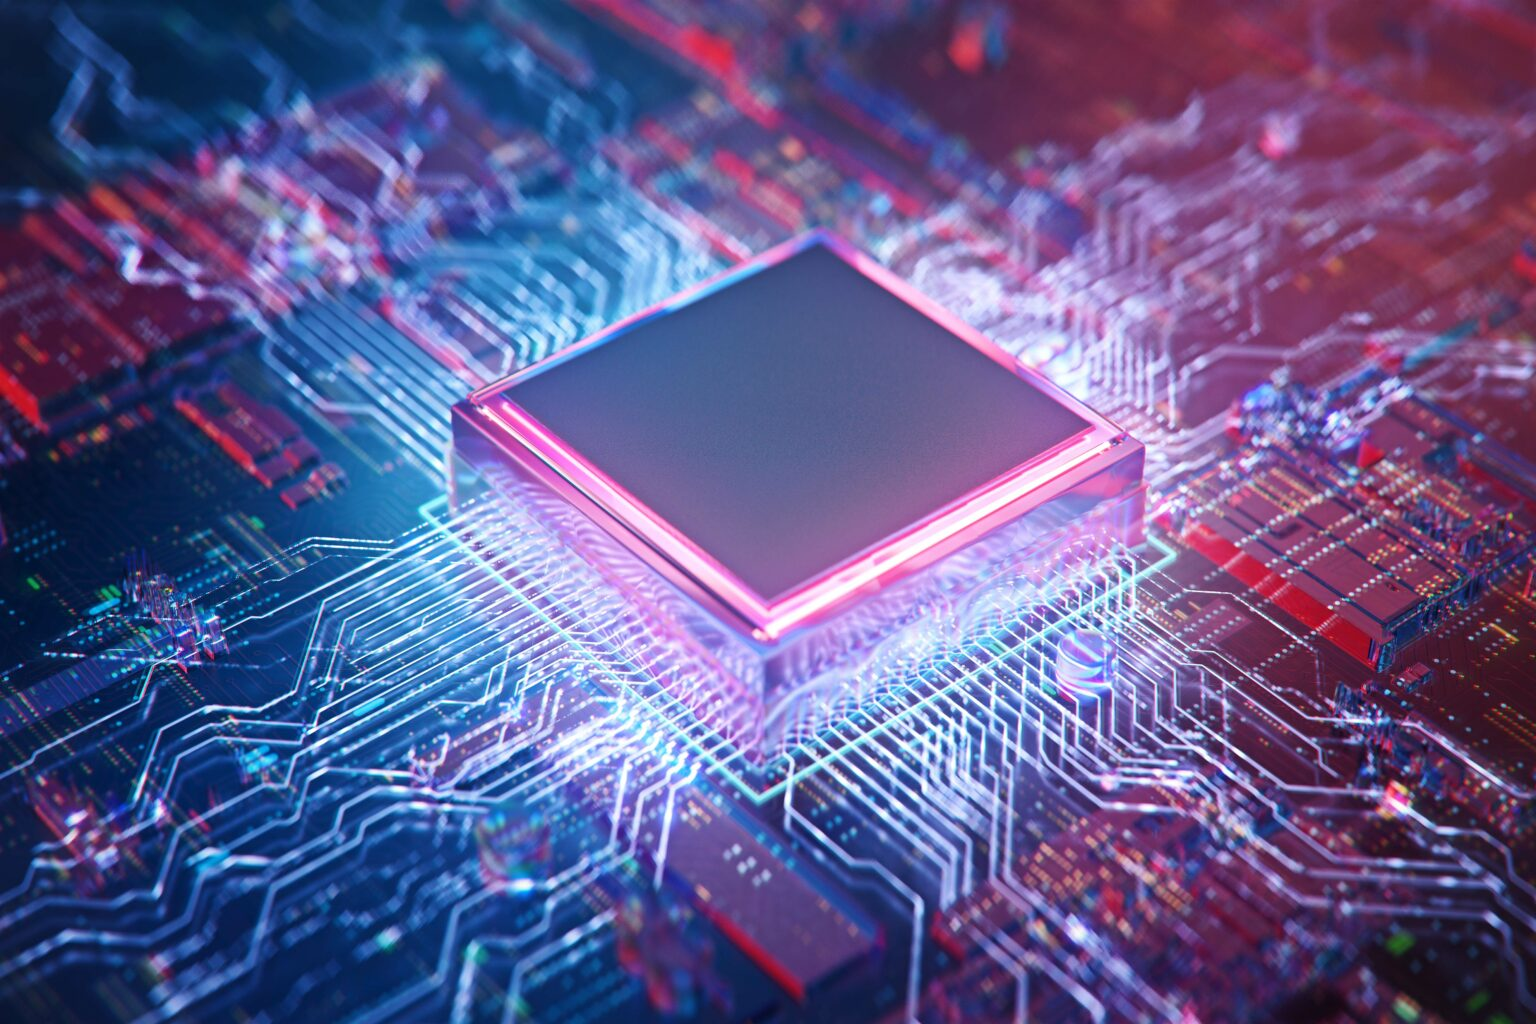
\includegraphics[height=6cm]{Cover/coverimage}};
        %adjust this coordinate to move image
      \end{tikzpicture}
    \end{center} % gráficos

    \vspace{5mm}
    \centering
    \LARGE \textbf{Memristors-based recurent modules for neural computing}
    \\ \vspace{15mm}
    \Large \textbf{Valentin BARBAZA} \\
    \vspace{12mm}
    \large Thesis to obtain the Master of Science Degree in
    \\ \vspace{2mm}
    \LARGE \textbf{Electrical and Computer Engineering}
    \\ \vspace{10mm}
    \large Supervisors: Dr. Diogo Caetano \\
    \large Dr. Ruxandra Barbulescu
    \\ \vspace{15mm}
    \Large \textbf{Examinatiom Committee}
    \\ \vspace{5mm}
    \large Chairperson: Prof. Lorem \\
    \large Supervisor: Prof. Lorem Ipsum\\
    \large Co-Supervisor: Prof. Lorem Ipsum \\
    \large Members of the Committe: Dr. Lorem Ipsum \\
    Prof. Lorem Ipsum

    \vspace{10mm}

    %\Large \textbf{\todaythesis\today} \\
    \Large \textbf{July/October 2023} \\
    \let\thepage\relax
  \end{flushleft}
  \pagebreak


  \clearpage
  % Since I am using double sided pages, the second page should be white.
  % Remember that when delivering the dissertation, IST requires for the cover to appear twice.

  \thispagestyle{empty}
  \cleardoublepage

  \setcounter{page}{1} \pagenumbering{roman}

  \baselineskip 18pt % line spacing: -12pt for single spacing
  %               -18pt for 1 1/2 spacing
  %               -24pt for double spacingnts}
 
%\thispagestyle{empty}
\hbox{} \vfill
\begin{flushright}
\small \textit{\textbf{Anyone who has never made a mistake has never tried anything new.}}
\\ \vspace{2mm}  
\scriptsize Albert Einstein
\end{flushright}

\clearpage
\thispagestyle{empty}
\cleardoublepage

\pdfbookmark{Acknowledgments}{Acknowledgments}
\begin{acknowledgments} 

I would like to thank the Academy, bla bla bla..

\end{acknowledgments}
\clearpage
\thispagestyle{empty}
\cleardoublepage
\begin{abstract}

The Objective of this Work ... (English)

\end{abstract}
\begin{keywords}
Memristors, Crossbar array, RNN, LSTM, Analog
\end{keywords}
\clearpage
\thispagestyle{empty}
\cleardoublepage
%\begin{resumo}

O objectivo deste trabalho ... (Português)

\end{resumo}
%\begin{palavraschave}
Palavras-Chave (Português)
\end{palavraschave}
\clearpage
\thispagestyle{empty}
\cleardoublepage
% This is required for the fancy chapters
\dominitoc
\dominilof
\dominilot

%%%%%%%%%%%%%%%%%%%%%%%%%%%%%%%%%%%%%%%%%%%%%%%%%%%%%%%%%%%%%%%%%%%%%%
% List of contents
%\renewcommand{\baselinestretch}{1}
\pdfbookmark[0]{Index}{index}
\pdfbookmark[1]{Contents}{toc}
\tableofcontents
% \contentsline{chapter}{References}{\pageref{bib}}
\clearpage
\thispagestyle{empty}
\cleardoublepage
%\renewcommand{\baselinestretch}{1.5}
%%%%%%%%%%%%%%%%%%%%%%%%%%%%%%%%%%%%%%%%%%%%%%%%%%%%%%%%%%%%%%%%%%%%%%
% List of figures
\pdfbookmark[1]{List of Figures}{lof}
\listoffigures
\clearpage
\thispagestyle{empty}
\cleardoublepage

%%%%%%%%%%%%%%%%%%%%%%%%%%%%%%%%%%%%%%%%%%%%%%%%%%%%%%%%%%%%%%%%%%%%%%
% List of tables
\pdfbookmark[1]{List of Tables}{lot}
\listoftables
\clearpage
\thispagestyle{empty}
\cleardoublepage

% %%%%%%%%%%%%%%%%%%%%%%%%%%%%%%%%%%%%%%%%%%%%%%%%%%%%%%%%%%%%%%%%%%%%%%
% % List of algorithms
% Requires packages algorithmic, algorithm
% \pdfbookmark[1]{List of Algorithms}{loa}
% \listofalgorithms
% \cleardoublepage
\acresetall
% %%%%%%%%%%%%%%%%%%%%%%%%%%%%%%%%%%%%%%%%%%%%%%%%%%%%%%%%%%%%%%%%%%%%%%
% List of acronyms
\pdfbookmark[1]{List of Acronyms}{loac}

\chapter*{Abbreviations}


% See more at http://staff.science.uva.nl/~polko/HOWTO/LATEX/acronym.html

\begin{acronym}
  \acro{AI}{Artifical Intelligence}
  \acro{NN}{Neural Network}
  \acro{VMM}{Vector Matrix Multiplication}
  \acro{opamp}{operational amplifier}
  \acro{LSTM}{Long Short-Term Memory}
  \acro{RNN}{Recurrent Neural Network}
  \acro{VMM}{Vector Matrix Multiplication}
  \acro{CPU}{Central Processing Unit}
  \acro{GPU}{Graphics Processing Unit}
  \acro{FPGA}{Field Programmable Gate Array}
  \acro{ASIC}{Application-Specific Integrated Circuit}
  \acro{NP}{No Peephole}
  \acro{FGR}{Full Gate Recurrence}
  \acro{CIFG}{Coupled Input-Forget Gate}
  \acro{GRU}{Gated Recurrent Unit}
\end{acronym}

\clearpage
\thispagestyle{empty}
\cleardoublepage




%%%%%%%%%%%%%%%%%%%%%%%%%%%%%%%%%%%%%%%%%%%%%%%%%%%%%%%%%%%%%%%%%%%%%%
% List of symbols
\pdfbookmark[1]{List of Symbols}{los}

\listofsymbols

\clearpage
\thispagestyle{empty}

\cleardoublepage
% Pages number is starting now with arabic style... until now it was on roman mode
\pagenumbering{arabic} \setcounter{page}{1}
\baselineskip 18pt
%\pagestyle{document}%Fancy head and foot with lines
\pagestyle{documentsimple}%Simple head
% %%%%%%%%%%%%%%%%%%%%%%%%%%%%%%%%%%%%%%%%%%%%%%%%%%%%%%%%%%%%%%%%%%%%%%
% The Introduction:
% %%%%%%%%%%%%%%%%%%%%%%%%%%%%%%%%%%%%%%%%%%%%%%%%%%%%%%%%%%%%%%%%%%%%%%
\fancychapter{Introduction}
\label{cap:int}

\section{Motivation}
\label{sec:int_motivation}

Nowadays, it's impossible not to have heard about \acp{AI}, they are everywhere and everybody talks about them. The most recent example being \textit{ChatGPT} from \textbf{OpenAI} and is getting very popular even outside of the "computer community"(TODO : Find better term). Everybody is using those tools. It's clear that \ac{AI} is becoming more and more important in the current world. 

\ac{AI} is wide topic, usually when we talk about \acp{AI}, we refer to the most common type, Machine Learning. Especially, a sub part of Machine Learning called Deep Learning. Deep Learning has seen a surge in research the last decade, which lead to great advancement in this field and the numerous \ac{AI} tools that popped up in the last years.
Deep Learning works using what is called \acp{NN}.

Those \acp{NN} require matrix multiplication. This kind of operation is very time and energy consuming to run on a classic computer. There are options to better run those operations. GPUs can be better suited than a CPU for a \ac{NN} application as it is made for 3D graphics that also mainly use Matrix Multiplication. Other specialized hardware such as FPGAs and ASICs can improve both execution time and energy consumption. All those are digital computers, using analog computing could highly improve speed, power consumption and even smaller chip area. All this using a memristive crossbar array \cite{Xbar}. An analog computer 
The point of this thesis is to lay out the ground work to create a LSTM capable chip to use in embedded systems. It could be used detection and prediction of any kind of sequential events.
Using those memristors \cite{TheoMemristor}, which work like resistance with a memory component to them, that means that they can be set to a desired value.

\subsection{Neural Networks}\label{sec:nn}

\acfp{NN} are a network of several layers of artificial neurons. Figure \ref{fig:snn}, shows a simple representation of a \ac{NN}, the artificial neurons are the represented by the colored circles. On figure \ref{fig:snn} each arrow represent a synapse.

\begin{figure}[h!]
    \centering
    \includesvg[height=8cm]{Figures/Colored_neural_network.svg}
    \caption{Simple \acl{NN}}
    \label{fig:snn}
\end{figure}



They are several layers to a \ac{NN} : 
\begin{itemize}
    \item Input layer : This layer is simply the different inputs.
    \item Hidden layer : This layer can be (and usually is) wider than the one in figure \ref{fig:snn}, it is there to add more layers and thus more precision to the result
    \item Output layer : This layer is where you can find the result from the \ac{NN}.
\end{itemize}

In a computational \ac{NN}, synapses are represented by weights. Those weights are to be multiplied by the last neuron and then added to each other to produce the next stage. Using the names defined in figure \ref{fig:nn_explained}, the equation linking each layer is the following matrix multiplication : 
\begin{equation}
    \begin{bmatrix}
    H1\\ H2\\ H3\\ H4\\
    \end{bmatrix}
    =
    \begin{bmatrix}
        W1,1 & W1,2 & W1,3\\
        W2,1 & W2,2 & W2,3\\
        W3,1 & W3,2 & W3,3\\
        W4,1 & W4,2 & W4,3\\
    \end{bmatrix}
    \cdot
    \begin{bmatrix}
        I1\\ I2\\ I3\\
    \end{bmatrix}
\end{equation}

And it works the same way to go to the next layer.

\begin{figure}[h!]
    \centering
    \includesvg[height=8cm]{Figures/NN_explained.svg}
    \caption{\aclp{NN} with names}
    \label{fig:nn_explained}
\end{figure}

Those matrix multiplication are very power-hungry and their computation time scales up with the size of the \ac{NN} using classical computing.

Analog computation enables those same calculations almost instantly and being far more power-efficient. This can be done using the physical properties of electrical devices.
We want to reproduce one of those neural network using electrical circuits to perform the same computation that a computer would in much faster manner.
Using \hyperref[subsec:memristors]{memristors} as weights. This removes the need to copy the weights from the main memory
\section{State of The Art}
\label{sec:int_state}

\subsection{Memristors}\label{subsec:memristors}

Memristors are the lesser known fourth fundamental passive component of electronics, among resistors, capacitors and inductor.
It was first theorized in 1971 by L. Chua from UC Berkeley, in \cite{TheoMemristor}. The name comes from the blend of \textit{memory} and \textit{resistance}.
The theory behind the component was extracted from a missing component to link the fundamental circuit variables. In figure \ref{fig:fundComp}, the four fundamental variables are on each side of the square, with the ones on opposite sides being linked as shown in the following equations :
\begin{equation}
  d\phi = v\cdot dt
\end{equation}

\begin{equation}
  dq = i\cdot dt
\end{equation}
Resistors, capacitors and inductors were already discovered and well known, so it was theorized that a fourth device should then exists to physically link flux ($\phi$) and charge ($q$).  The flux in this case is not a magnetic flux and is defined as such : $ d\phi=V\cdot dt \implies \phi =  \int V(t) \,dt  $.\\
The component stayed theoretical until 2008 when it's been implemented in a physical device for the first time \cite{Strukov2008}. It took 37 years to actually have a working device.\\
There is then an extention of this theoretical device to another, the memristive device. It was theorized in 1976 by L. Chua and S. M. Kang \cite{memrestiveDev}. The difference between the memristor and the memristive device is its internal behavior. Memristive device are commonly referred to as memristor as well.

\begin{figure}[H]
  \centering
  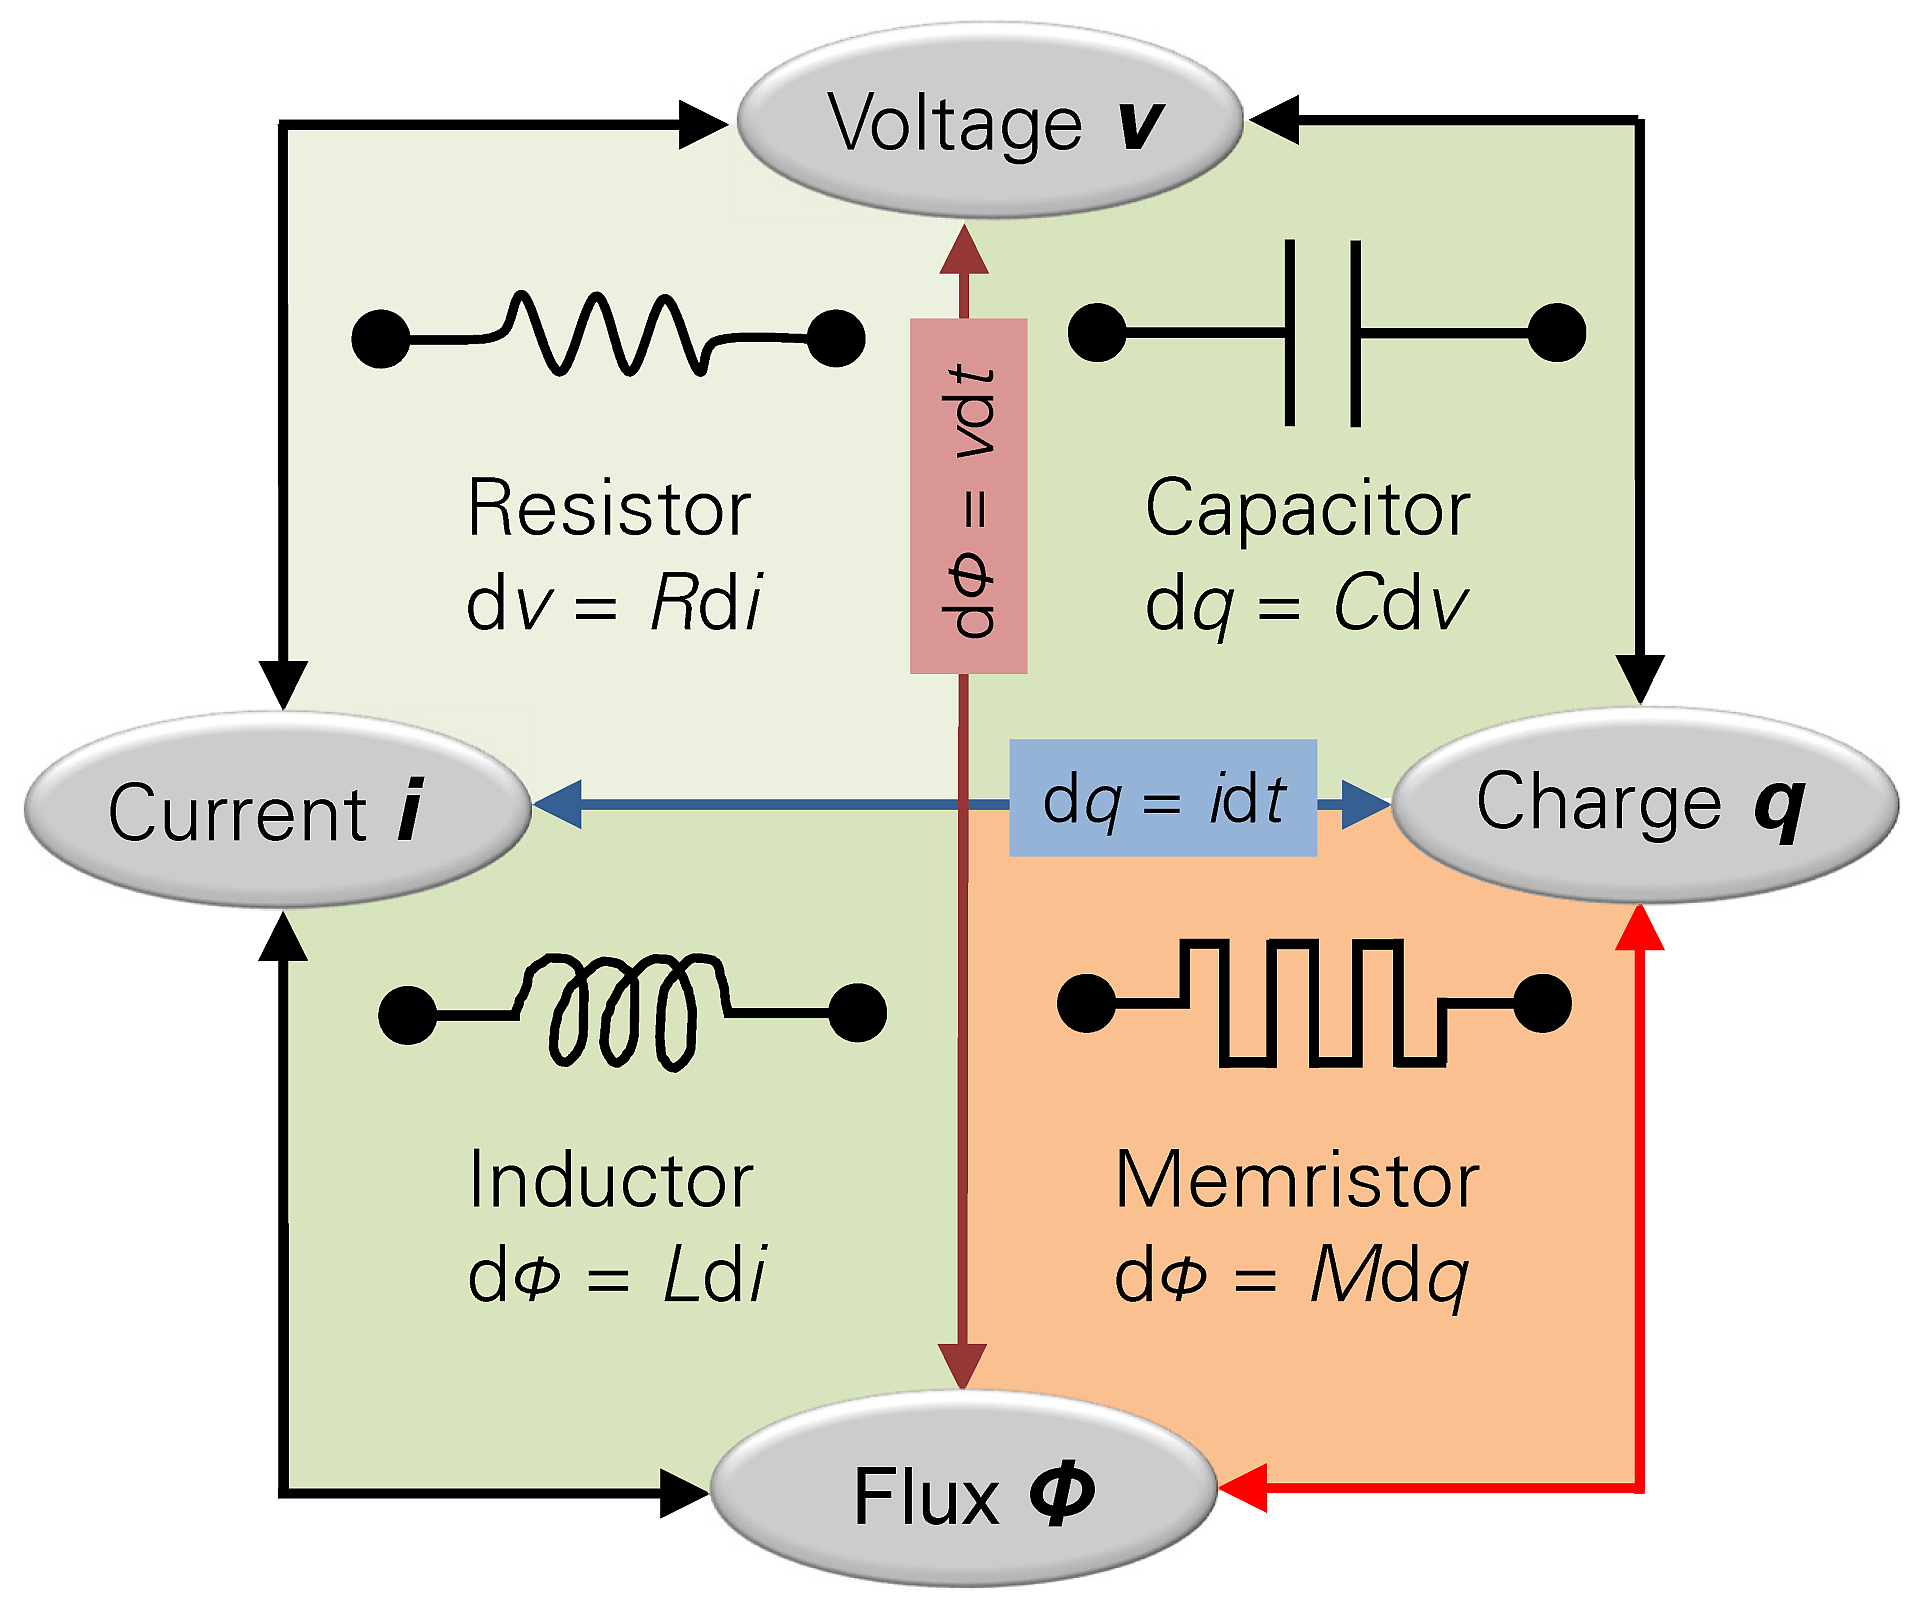
\includegraphics{Figures/Memristor.png}
  \caption{Fundamental passive components}
  \label{fig:fundComp}
\end{figure}

\subsubsection{Equations}
A memristor links the flux ($\phi$) and charge ($q$) and creates the memristance.
This memristance is defined with the following equation :
\begin{equation}
  M(q)=\frac{d\phi}{dq}
\end{equation}
It can be compared with the other fundamental components like resistor ($R(i)=\frac{dv}{di}$), capacitor ($\frac{1}{C(q)}=\frac{dv}{dq}$) and inductor ($L(i)=\frac{d\phi}{di}$).
We can then extract a more useful equation in an actual circuit :
\begin{equation}
  v(t)=M(q(t))\cdot i(t)
\end{equation}
Similarly, a memductance can be defined as such :
\begin{equation}
  W(\phi)=\frac{dq}{d\phi}
\end{equation}
A memristive device is slightly differently defined, it still uses a memristance, but here the memristance also depends on an internal state called $x$. This gives us this equation :
\begin{equation}
  v(t)=M(x,i)\cdot i(t)
\end{equation}
The internal state ($x$) is not linked to flux or charge in the case of a memristive device.\\
Once again, we can also define the memristive device using a memductance :
\begin{equation}
  i(t)=W(x,v)\cdot v(t)
\end{equation}
In all of the previous equations, $v$ is the voltage in Volt ($V$), $i$ is the current in Ampere ($A$), $\phi$ is the flux in Weber ($Wb$), $q$ is the charge in Coulomb ($C$), $M$ is the memristance in Ohm ($\Omega$) and $W$ is the memductance in Siesmens ($S$ or $\Omega^{-1}$).

\subsubsection{Behavior}
A memristor is defined as a non-linear two-terminal fundamental electrical component. It behaves as a resistance with memory (hence its name), meaning that it changes its resistance based on how much charge went through it. This enables us to manipulate the resistance of the component.
The huge benefit of memristors is the memory component, when you power it, it will have the resistance it had before.

Memristive devices have a similar behavior, the memristive device's resistance will change depending on the internal state ($x$). That internal state changes based on how much and how long voltage signals or currents are applied to the memristive device.

\subsubsection{Usage}
The main research for memristor usage is using them as ReRAM. The idea behind ReRAM is to use memristors as Non-Volatile memory. It uses two states of the device with known resistances ($R_{on}$ and $R_{off}$), giving it binary property. Reading the memory simply requires setting a voltage and reading the output current. It is better than current solutions (HDD, SSD) as it has a much lower latency. It is better than traditionnal DRAM because it keeps the information even when turned off. This makes ReRAM a good replacement for both RAM and HDDs/SSDs, thus eliminating Von Neumann bottleneck due to the Von Neumann architecture that is used in all modern computers.

They can also be used to set a resistance to be able to perform analog multiplication. Setting them in a crossbar array makes them a very strong candidate to be used in neuromorphic computing.

\subsection{Memristors Crossbar Array}\label{subsec:crossbar}

Setting memristors in a crossbar array to perform analog matrix multiplication typically called Multiply and Accumulate because of the nature of Matrix Multiplication. Figure \ref{fig:crossbar} shows what a typical crossbar array looks like.

\begin{figure}[H]
  \centering
  %\subfloat[Schematics]{\includesvg[width=.45\linewidth]{Figures/crossbar.svg}}\qquad
  \subfloat[Schematics]{
\includegraphics[width=.45\linewidth]{Figures/crossbar.eps}}%\qquad
  \hfill
  \subfloat[3 dimensional representation]{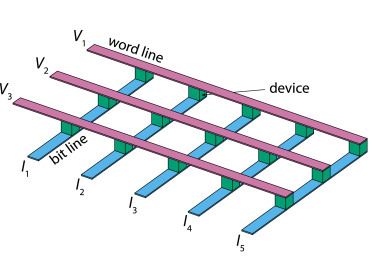
\includegraphics[width=.45\linewidth]{Figures/crossbar3D.jpg}}\\
  \caption{Memristor crossbar array}
  \label{fig:crossbar}
\end{figure}

It uses physical properties of electrical systems to perform analog computing. Lets use the circuit node in figure \ref{fig:crossNode} to explain the theory behind the memristor crossbar array.
\begin{figure}[H]
  \centering
  %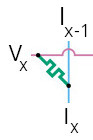
\includegraphics{Figures/crossbar-node.jpg}
  \includesvg[height=3.5cm]{Figures/crossbarNode.svg}
  \caption{Memristor crossbar node of the $i^{th}$ line and $j^{th}$ column}
  \label{fig:crossNode}
\end{figure}

First of all, a voltage is applied on the $i^{th}$ line, because every column is virtually grounded, the voltage applied to the memristor, of a set resistance of $R$, is $V_i$. As such and using Ohm's law, we know the the current flowing into the memristor is bound by the following equation :
\begin{equation}
  V_i = R\cdot I_{mem} \implies I_{mem} = V_i\cdot (\frac{1}{R})=I_{mem} = V_i\cdot G
\end{equation}
With $G$ being the conductance of memristor.
This line then joins the column where a current of $I_{i,j-1}$ is flowing, then according to kirchhoff's law the resulting current is :
\begin{equation}
  I_{j,i} = I_{j,i-1}+I_{mem} = I_{j,i-1} + V_i\cdot G
\end{equation}
By applying this process to the whole system we find that the current as the bottom of one column is :
\begin{equation}
  I_1=G_1\cdot V_1 + G_2\cdot V_2 + G_3\cdot V_3
\end{equation}
With $G_1$, $G_2$ and $G_3$ being the conductance of the 3 memristors in the first column.

This analog circuit removes the need to copy data from a main memory as the memristors themselves hold the value and the weights are then stored where the computation happens.

\subsection{memristor's model}
TODO
\subsection{LSTM}
\acp{LSTM} are a type of \ac{NN} used to analyze sequence of data. They are capable of predict data based of the previous results. \acp{LSTM} are part of \acp{RNN}. \acp{RNN} are different than feedfoward \acl{NN} because of their feedback connections. Meaning that the results from the last time step have an impact on the next time step.

\acp{LSTM} are able to forget information passed. This ability gave the uncommon name of \acl{LSTM} as it has both long and short term memory. This what gives \acp{LSTM} their use for sequence data. They can analyze the data and keep the information from the last time step to make a better decision afterwards. The most comprehensible example is considering a sentence. (TODO : find example)

An \ac{LSTM} is more complicated than just a simple feedforward \acl{NN}, they have several gates, which are all technically a \ac{NN} themselves. There is also a cell state which job is to hold a value for the next step.

\begin{figure}[H]
  \centering
  \includesvg[width=\textwidth]{Figures/lstmCellLatex.svg}
  \caption{LSTM Cell}
  \label{fig:lstmCell}
\end{figure}

Figure \ref{fig:lstmCell} shows the complexity of the \ac{LSTM} architecture. In an \ac{LSTM}, each gate is a different \ac{NN}.

An \ac{LSTM} works using different gates
\subsection{Dummy Subsection B}
\label{subsec:subsectionb}

State of Art Subsection B


\section{Original Contributions}
\label{sec:int_contributions}

Contributions Section.

\begin{figure}[H]
    \centering
    
\usetikzlibrary{ calc, positioning, decorations.markings, patterns}
% all other packages and stuff you need for the picture
%
\begin{tikzpicture}[thick]


  % Seperation between lines
  \pgfmathsetlengthmacro{\wavesep}{2.0em}

  % Height of a waveform
  \pgfmathsetlengthmacro{\waveheight}{1.2em}

  % Width of a brick (half a cycle)
  \pgfmathsetlengthmacro{\wavewidth}{1em}

  % Width of the slant on slanted signal changes
  \pgfmathsetlengthmacro{\transitionwidth}{0.3em}

  % Width of the curve on slow signal changes (e.g. to z)
  \pgfmathsetlengthmacro{\curvedtransitionwidth}{1.0em}

  % Special signal styles
  \tikzset{wave x/.style={pattern=north east lines}}
  \tikzset{wave bus/.style={fill=white}}
  \tikzset{wave busyellow/.style={fill=yellow!25!white}}
  \tikzset{wave busorange/.style={fill=orange!25!white}}
  \tikzset{wave busblue/.style={fill=blue!25!white}}
  \tikzset{wave pulled/.style={dotted}}

  % Initialise pointer
  \coordinate (last waveform);

  % Label for a signal. Arguments:
  %  #1: The human-readable label string
  \newcommand{\signallabel}[1]{
    \node [ anchor=east
    , left=0 of last waveform
    , minimum height=\waveheight
    ]
    {#1};
  }

  % Advance the "last brick" coordinate to the next position
  %  #1: Width of a brick
  \newcommand{\advancebrick}[1]{
    \coordinate (last brick) at ([shift={(#1*\wavewidth,0)}]last brick);
  }

  % Add the label for a bus
  %  #1: Label coordinate
  %  #2: Label text
  \newcommand{\busdata}[2]{
    \node [ inner sep=0
    , minimum height=\waveheight
    , anchor=mid
    , font=\footnotesize
    ]
    at ([shift={(0.5*\transitionwidth,0)}]#1)
    {#2};
  }

  % Define a clip which will truncate a waveform at the left-hand side
  %  #1: Width of a brick
  %  #2: Truncation offset (in bricks)
  %  #3: Number of bricks in waveform
  \newcommand{\truncatewaveform}[3]{
    \coordinate (last brick) at ([shift={(-#2*\wavewidth,0)}]last brick);
    \clip ([shift={(#2*\wavewidth, 0.6*\waveheight)}]last brick)
    rectangle ++(#3*#1*\wavewidth-#2*\wavewidth,-1.2*\waveheight);
  }

  % Spacer Brick Overlay
  %  #1: brick width
  \newcommand{\brickspaceroverly}[1]{
    \pgfmathsetlengthmacro{\spacerheight}{1.2*\waveheight}
    \pgfmathsetlengthmacro{\spacerwidth}{\transitionwidth}
    \pgfmathsetlengthmacro{\spacergap}{0.7*\transitionwidth}

    % Mask off the waveform
    \fill [fill=white]
    ([xshift=-#1*\wavewidth-0.5*\spacergap-0.5*\spacerwidth, yshift=-0.5*\spacerheight]last brick)
    .. controls +(0.8*\spacergap, 0) and +(-0.8*\spacergap, 0)
    .. ++(\spacerwidth, \spacerheight)
    -- ++(\spacergap,0)
    .. controls +(-0.8*\spacergap, 0) and +(0.8*\spacergap, 0)
    .. ++(-\spacerwidth, -\spacerheight)
    ;

    % Lines
    \draw ([xshift=-#1*\wavewidth-0.5*\spacergap-0.5*\spacerwidth, yshift=-0.5*\spacerheight]last brick)
    .. controls +(0.8*\spacergap, 0) and +(-0.8*\spacergap, 0)
    .. ++(\spacerwidth, \spacerheight)
    ++(\spacergap,0)
    .. controls +(-0.8*\spacergap, 0) and +(0.8*\spacergap, 0)
    .. ++(-\spacerwidth, -\spacerheight)
    ;

  }

  % Generic mid-bus brick
  %  #1: brick width
  %  #2: brick style
  \newcommand{\brickbus}[2]{
    \fill [#2]
    ([yshift= 0.5*\waveheight]last brick)
    -- ++(#1*\wavewidth,0)
    -- ++(0,-\waveheight)
    -- ++(-#1*\wavewidth,0)
    -- cycle
    ;
    \draw ([yshift= 0.5*\waveheight]last brick) -- ++(#1*\wavewidth,0)
    ([yshift=-0.5*\waveheight]last brick) -- ++(#1*\wavewidth,0)
    ;

    \advancebrick{#1}
  }

  % Generic mid-bit brick
  %  #1: brick width
  %  #2: Line style
  %  #3: Start line offset (from bottom)
  %  #4: End line offset (from bottom)
  %  #5: Add arrow on transition
  \newcommand{\brickbit}[5]{
    \pgfmathsetlengthmacro{\vstart}{(#3-0.5)*\waveheight}
    \pgfmathsetlengthmacro{\vend}{(#4-0.5)*\waveheight}

    % The bit value
    \draw [#2]
    ([yshift=\vend]last brick)
    |- ([yshift=\vstart, xshift=#1*\wavewidth]last brick);

    % Arrow (if required)
    \ifthenelse{\equal{#5}{1}}{
      \path [decoration={ markings
      , mark=at position 0.5 with {\arrow{>}}
      }
      , postaction={decorate}
      ]
      ([yshift=\vend]last brick)
      -- ([yshift=\vstart]last brick);
    }{}

    \advancebrick{#1}
  }

  % Generic bit-glitch brick
  %  #1: brick width
  %  #2: Style
  %  #3: Edge start (offset from bottom)
  \newcommand{\brickbitglitch}[3]{
    \pgfmathsetlengthmacro{\voffset}{(#3-0.5)*\waveheight}

    \draw [#2]
    ([yshift=\voffset]last brick)
    -- ([xshift=0.5*\transitionwidth]last brick)
    -- ([yshift=\voffset, xshift=\transitionwidth]last brick)
    -- ++(#1*\wavewidth - \transitionwidth,0);

    \advancebrick{#1}
  }

  % Generic sharp bit-to-bit transition
  %  #1: brick width
  %  #2: Brick style
  %  #3: Old bit (offset from bottom)
  %  #4: New bit (offset from bottom)
  %  #5: Include arrow
  \newcommand{\bricksharpbittobit}[5]{
    \pgfmathsetlengthmacro{\vstart}{(#3-0.5)*\waveheight}
    \pgfmathsetlengthmacro{\vend}{(#4-0.5)*\waveheight}

    % The transition and new bit
    \draw [#2]
    ([yshift=\vstart]last brick)
    -- ([yshift=\vend]last brick)
    -- ++(#1*\wavewidth,0);

    % Arrow (if required)
    \ifthenelse{\equal{#5}{1}}{
      \ifthenelse{\not\equal{#3}{#4}}{
        \path [decoration={ markings
        , mark=at position 0.5 with {\arrow{>}}
        }
        , postaction={decorate}
        ]
        ([yshift=\vstart]last brick)
        -- ([yshift=\vend]last brick);
      }{}
    }{}

    \advancebrick{#1}
  }

  % Generic sharp bus-to-bit transition
  %  #1: brick width
  %  #2: Brick style
  %  #3: New bit (offset from bottom)
  %  #4: Include arrow
  \newcommand{\bricksharpbustobit}[4]{
    \pgfmathsetlengthmacro{\vstart}{((1-#3)-0.5)*\waveheight}
    \pgfmathsetlengthmacro{\vend}{(#3-0.5)*\waveheight}

    % The transition and new bit
    \draw [#2]
    ([yshift=\vstart]last brick)
    -- ([yshift=\vend]last brick)
    -- ++(#1*\wavewidth,0);

    % Arrow (if required)
    \ifthenelse{\equal{#4}{1}}{
      \path [decoration={ markings
      , mark=at position 0.5 with {\arrow{>}}
      }
      , postaction={decorate}
      ]
      ([yshift=\vstart]last brick)
      -- ([yshift=\vend]last brick);
    }{}

    \advancebrick{#1}
  }

  % Generic soft bit-to-bit transition
  %  #1: brick width
  %  #2: Last brick style
  %  #3: This brick style
  %  #4: Last bit (offset from bottom)
  %  #5: New bit (offset from bottom)
  \newcommand{\bricksmoothbittobit}[5]{
    \pgfmathsetlengthmacro{\vstart}{(#4-0.5)*\waveheight}
    \pgfmathsetlengthmacro{\vend}{(#5-0.5)*\waveheight}

    % Scale the transition depending on the magnitude of the level change
    \pgfmathsetlengthmacro{\thistranswidth}{abs(#4-#5)*\transitionwidth}
    \pgfmathsetlengthmacro{\thisleadwidth}{\transitionwidth - \thistranswidth}

    % The lead up to the transition
    \draw [#2]
    ([yshift=\vstart]last brick)
    -- ([yshift=\vstart, xshift=\thisleadwidth]last brick);

    % The transition itself
    \draw [#3]
    ([yshift=\vstart, xshift=\thisleadwidth]last brick)
    -- ([yshift=\vend, xshift=\transitionwidth]last brick)
    -- ++(#1*\wavewidth - \transitionwidth,0);

    \coordinate (last transition) at ([xshift=0.5*\transitionwidth]last brick);

    \advancebrick{#1}
  }

  % Generic curved bit-to-bit transition
  %  #1: brick width
  %  #2: Last brick style
  %  #3: This brick style
  %  #4: Last bit (offset from bottom)
  %  #5: New bit (offset from bottom)
  \newcommand{\brickcurvedbittobit}[5]{
    \pgfmathsetlengthmacro{\vstart}{(#4-0.5)*\waveheight}
    \pgfmathsetlengthmacro{\vend}{(#5-0.5)*\waveheight}

    % The curve itself
    \draw [#2]
    ([yshift=\vstart]last brick)
    .. controls ([yshift=\vstart]last brick)
    and ([yshift=\vend, xshift=0.2*\curvedtransitionwidth]last brick)
    .. ([yshift=\vend, xshift=\curvedtransitionwidth]last brick);

    % Start of the new bit
    \draw [#3]
    ([yshift=\vend, xshift=\curvedtransitionwidth]last brick)
    -- ++(#1*\wavewidth - \curvedtransitionwidth,0);

    \coordinate (last transition) at ([xshift=0.5*\curvedtransitionwidth]last brick);

    \advancebrick{#1}
  }

  % Generic soft transition from bit to bus
  %  #1: brick width
  %  #2: Bit style
  %  #3: Bus style
  %  #4: Bit (offset from bottom)
  \newcommand{\bricksmoothbittobus}[4]{
    \pgfmathsetlengthmacro{\voffset}{(#4-0.5)*\waveheight}

    % Scale the transition depending on the magnitude of the level change
    \pgfmathsetlengthmacro{\thistranswidth}{(abs(#4-0.5)+0.5)*\transitionwidth}
    \pgfmathsetlengthmacro{\thisleadwidth}{\transitionwidth - \thistranswidth}

    % The lead up to the transition
    \draw [#2]
    ([yshift=\voffset]last brick)
    -- ([yshift=\voffset, xshift=\thisleadwidth]last brick);

    % Open-up the bus
    \draw [#3]
    ([xshift=#1*\wavewidth,    yshift= 0.5*\waveheight]last brick)
    -- ([xshift=\transitionwidth, yshift= 0.5*\waveheight]last brick)
    -- ([xshift=\thisleadwidth,   yshift=     \voffset]   last brick)
    -- ([xshift=\transitionwidth, yshift=-0.5*\waveheight]last brick)
    -- ([xshift=#1*\wavewidth,    yshift=-0.5*\waveheight]last brick)
    ;

    \coordinate (last transition) at ([xshift=0.5*\transitionwidth]last brick);

    \advancebrick{#1}
  }

  % Generic smooth transition from bus to bus
  %  #1: brick width
  %  #2: Bus style
  %  #3: Bit style
  \newcommand{\brickbustobus}[3]{

    % Close-down the old bus
    \draw [#2]
    ([yshift= 0.5*\waveheight]    last brick)
    -- ([xshift=0.5*\transitionwidth]last brick)
    -- ([yshift=-0.5*\waveheight]    last brick)
    ;

    % Open-up the new bus
    \draw [#3]
    ([xshift=#1*\wavewidth,    yshift= 0.5*\waveheight]last brick)
    -- ([xshift=\transitionwidth, yshift= 0.5*\waveheight]last brick)
    -- ([xshift=0.5*\transitionwidth]                     last brick)
    -- ([xshift=\transitionwidth, yshift=-0.5*\waveheight]last brick)
    -- ([xshift=#1*\wavewidth,    yshift=-0.5*\waveheight]last brick)
    ;

    \coordinate (last transition) at ([xshift=0.5*\transitionwidth]last brick);

    \advancebrick{#1}
  }

  % Generic smooth transition from bus to bit
  %  #1: brick width
  %  #2: Bus style
  %  #3: Bit style
  %  #4: Bit (offset from bottom)
  \newcommand{\bricksmoothbustobit}[4]{
    \pgfmathsetlengthmacro{\voffset}{(#4-0.5)*\waveheight}

    % Scale the transition depending on the magnitude of the level change
    \pgfmathsetlengthmacro{\thistranswidth}{(abs(#4-0.5)+0.5)*\transitionwidth}
    \pgfmathsetlengthmacro{\thisleadwidth}{\transitionwidth - \thistranswidth}

    % Close-down the bus
    \draw [#2]
    ([                         yshift= 0.5*\waveheight]last brick)
    -- ([xshift=\thisleadwidth,   yshift= 0.5*\waveheight]last brick)
    -- ([xshift=\transitionwidth, yshift=     \voffset]   last brick)
    -- ([xshift=\thisleadwidth,   yshift=-0.5*\waveheight]last brick)
    -- ([                         yshift=-0.5*\waveheight]last brick)
    ;

    % The new bit
    \draw [#3]
    ([xshift=\transitionwidth, yshift=\voffset]last brick)
    -- ([xshift=#1*\wavewidth,    yshift=\voffset]last brick);

    \coordinate (last transition) at ([xshift=0.5*\transitionwidth]last brick);

    \advancebrick{#1}
  }

  % Generic curved transition from bus to bit
  %  #1: brick width
  %  #2: Bus style
  %  #3: Bit style
  %  #4: Bit (offset from bottom)
  \newcommand{\brickcurvedbustobit}[4]{
    \pgfmathsetlengthmacro{\voffset}{(#4-0.5)*\waveheight}

    % Scale the transition depending on the magnitude of the level change
    \pgfmathsetlengthmacro{\thistranswidth}{(abs(#4-0.5)+0.5)*\transitionwidth}
    \pgfmathsetlengthmacro{\thisleadwidth}{\transitionwidth - \thistranswidth}

    % Close-down the bus
    \draw [#2]
    ([yshift= 0.5*\waveheight]last brick)
    .. controls ([                                   yshift= 0.5*\waveheight]last brick)
    and ([xshift=0.2*\curvedtransitionwidth, yshift=     \voffset]   last brick)
    .. ([xshift=\curvedtransitionwidth, yshift= \voffset]last brick)
    .. controls ([xshift=0.2*\curvedtransitionwidth, yshift=     \voffset]   last brick)
    and ([                                   yshift=-0.5*\waveheight]last brick)
    .. ([yshift=-0.5*\waveheight]last brick)
    ;

    % The new bit
    \draw [#3]
    ([xshift=\curvedtransitionwidth, yshift=\voffset]last brick)
    -- ([xshift=#1*\wavewidth,    yshift=\voffset]last brick);

    \coordinate (last transition) at ([xshift=0.5*\curvedtransitionwidth]last brick);

    \advancebrick{#1}
  }

  \foreach \tick in {0,...,13}{
    \draw [draw=black!75!white, dotted]
    ([xshift=\tick*2.0*\wavewidth,yshift=0.5*\waveheight]last waveform)
    -- ++(0, -6*\wavesep + \wavesep - \waveheight);
  }

  \signallabel{}
  % A scope to ensure correct styling and limit the effect of clipping
  \begin{scope}[line cap=rect, line join=round]

  \end{scope}
  \coordinate (last waveform) at ([yshift=-\wavesep]last waveform);


  \signallabel{cycles}
  % A scope to ensure correct styling and limit the effect of clipping
  \begin{scope}[line cap=rect, line join=round]
    \coordinate (last brick) at (last waveform);
    \coordinate (last transition) at (last brick);
    \brickbus{1.000000}{wave x}
    \brickbus{1.000000}{wave x}
    \coordinate (last transition) at (last brick);
    \coordinate (bus start) at (last brick);
    \brickbustobus{1.000000}{wave x}{wave bus}
    \brickbus{1.000000}{wave bus}
    \coordinate (G) at (last transition);
    \coordinate (last transition) at (last brick);
    \brickbus{1.000000}{wave bus}
    \brickbus{1.000000}{wave bus}
    \coordinate (last transition) at (last brick);
    \brickbus{1.000000}{wave bus}
    \brickbus{1.000000}{wave bus}
    \coordinate (last transition) at (last brick);
    \brickbus{1.000000}{wave bus}
    \brickbus{1.000000}{wave bus}
    \coordinate (last transition) at (last brick);
    \brickbus{1.000000}{wave bus}
    \brickbus{1.000000}{wave bus}
    \coordinate (last transition) at (last brick);
    \coordinate (bus 0) at ($(bus start)!0.5!(last brick)$);
    \coordinate (bus start) at (last brick);
    \brickbustobus{1.000000}{wave bus}{wave bus}
    \brickbus{1.000000}{wave bus}
    \coordinate (H) at (last transition);
    \coordinate (last transition) at (last brick);
    \brickbus{1.000000}{wave bus}
    \brickbus{1.000000}{wave bus}
    \brickspaceroverly{1.000000}
    \coordinate (last transition) at (last brick);
    \coordinate (bus 1) at ($(bus start)!0.5!(last brick)$);
    \coordinate (bus start) at (last brick);
    \brickbustobus{1.000000}{wave bus}{wave bus}
    \brickbus{1.000000}{wave bus}
    \coordinate (last transition) at (last brick);
    \brickbus{1.000000}{wave bus}
    \brickbus{1.000000}{wave bus}
    \coordinate (last transition) at (last brick);
    \brickbus{1.000000}{wave bus}
    \brickbus{1.000000}{wave bus}
    \coordinate (last transition) at (last brick);
    \brickbus{1.000000}{wave bus}
    \brickbus{1.000000}{wave bus}
    \coordinate (last transition) at (last brick);
    \brickbus{1.000000}{wave bus}
    \brickbus{1.000000}{wave bus}
    \coordinate (bus 2) at ($(bus start)!0.5!(last brick)$);
    \busdata{bus 0}{$cycle_1$};
    \busdata{bus 1}{};
    \busdata{bus 2}{$cycle_i$};
  \end{scope}
  \coordinate (last waveform) at ([yshift=-\wavesep]last waveform);


  \signallabel{$e_0$}
  % A scope to ensure correct styling and limit the effect of clipping
  \begin{scope}[line cap=rect, line join=round]
    \coordinate (last brick) at (last waveform);
    \coordinate (last transition) at (last brick);
    \brickbus{1.000000}{wave x}
    \brickbus{1.000000}{wave x}
    \coordinate (last transition) at (last brick);
    \bricksmoothbustobit{1.000000}{wave x}{}{1.000000}
    \brickbit{1.000000}{}{1.000000}{1.000000}{0}
    \coordinate (last transition) at (last brick);
    \bricksmoothbittobit{1.000000}{}{}{1.000000}{0.000000}
    \brickbit{1.000000}{}{0.000000}{0.000000}{0}
    \coordinate (last transition) at (last brick);
    \brickbit{1.000000}{}{0.000000}{0.000000}{0}
    \brickbit{1.000000}{}{0.000000}{0.000000}{0}
    \brickspaceroverly{1.000000}
    \coordinate (last transition) at (last brick);
    \brickbit{1.000000}{}{0.000000}{0.000000}{0}
    \brickbit{1.000000}{}{0.000000}{0.000000}{0}
    \coordinate (last transition) at (last brick);
    \brickbit{1.000000}{}{0.000000}{0.000000}{0}
    \brickbit{1.000000}{}{0.000000}{0.000000}{0}
    \coordinate (last transition) at (last brick);
    \coordinate (bus start) at (last brick);
    \bricksmoothbittobus{1.000000}{}{wave bus}{0.000000}
    \brickbus{1.000000}{wave bus}
    \coordinate (last transition) at (last brick);
    \brickbus{1.000000}{wave bus}
    \brickbus{1.000000}{wave bus}
    \brickspaceroverly{1.000000}
    \coordinate (last transition) at (last brick);
    \coordinate (bus 0) at ($(bus start)!0.5!(last brick)$);
    \bricksmoothbustobit{1.000000}{wave bus}{}{1.000000}
    \brickbit{1.000000}{}{1.000000}{1.000000}{0}
    \coordinate (last transition) at (last brick);
    \bricksmoothbittobit{1.000000}{}{}{1.000000}{0.000000}
    \brickbit{1.000000}{}{0.000000}{0.000000}{0}
    \coordinate (last transition) at (last brick);
    \brickbit{1.000000}{}{0.000000}{0.000000}{0}
    \brickbit{1.000000}{}{0.000000}{0.000000}{0}
    \brickspaceroverly{1.000000}
    \coordinate (last transition) at (last brick);
    \brickbit{1.000000}{}{0.000000}{0.000000}{0}
    \brickbit{1.000000}{}{0.000000}{0.000000}{0}
    \coordinate (last transition) at (last brick);
    \brickbit{1.000000}{}{0.000000}{0.000000}{0}
    \brickbit{1.000000}{}{0.000000}{0.000000}{0}
  \end{scope}
  \coordinate (last waveform) at ([yshift=-\wavesep]last waveform);


  \signallabel{$e_1$}
  % A scope to ensure correct styling and limit the effect of clipping
  \begin{scope}[line cap=rect, line join=round]
    \coordinate (last brick) at (last waveform);
    \coordinate (last transition) at (last brick);
    \brickbus{1.000000}{wave x}
    \brickbus{1.000000}{wave x}
    \coordinate (last transition) at (last brick);
    \bricksmoothbustobit{1.000000}{wave x}{}{0.000000}
    \brickbit{1.000000}{}{0.000000}{0.000000}{0}
    \coordinate (last transition) at (last brick);
    \bricksmoothbittobit{1.000000}{}{}{0.000000}{1.000000}
    \brickbit{1.000000}{}{1.000000}{1.000000}{0}
    \coordinate (last transition) at (last brick);
    \brickbit{1.000000}{}{1.000000}{1.000000}{0}
    \brickbit{1.000000}{}{1.000000}{1.000000}{0}
    \brickspaceroverly{1.000000}
    \coordinate (last transition) at (last brick);
    \bricksmoothbittobit{1.000000}{}{}{1.000000}{0.000000}
    \brickbit{1.000000}{}{0.000000}{0.000000}{0}
    \coordinate (last transition) at (last brick);
    \brickbit{1.000000}{}{0.000000}{0.000000}{0}
    \brickbit{1.000000}{}{0.000000}{0.000000}{0}
    \coordinate (last transition) at (last brick);
    \coordinate (bus start) at (last brick);
    \bricksmoothbittobus{1.000000}{}{wave bus}{0.000000}
    \brickbus{1.000000}{wave bus}
    \coordinate (last transition) at (last brick);
    \brickbus{1.000000}{wave bus}
    \brickbus{1.000000}{wave bus}
    \brickspaceroverly{1.000000}
    \coordinate (last transition) at (last brick);
    \coordinate (bus 0) at ($(bus start)!0.5!(last brick)$);
    \bricksmoothbustobit{1.000000}{wave bus}{}{0.000000}
    \brickbit{1.000000}{}{0.000000}{0.000000}{0}
    \coordinate (last transition) at (last brick);
    \bricksmoothbittobit{1.000000}{}{}{0.000000}{1.000000}
    \brickbit{1.000000}{}{1.000000}{1.000000}{0}
    \coordinate (last transition) at (last brick);
    \brickbit{1.000000}{}{1.000000}{1.000000}{0}
    \brickbit{1.000000}{}{1.000000}{1.000000}{0}
    \brickspaceroverly{1.000000}
    \coordinate (last transition) at (last brick);
    \bricksmoothbittobit{1.000000}{}{}{1.000000}{0.000000}
    \brickbit{1.000000}{}{0.000000}{0.000000}{0}
    \coordinate (last transition) at (last brick);
    \brickbit{1.000000}{}{0.000000}{0.000000}{0}
    \brickbit{1.000000}{}{0.000000}{0.000000}{0}
  \end{scope}
  \coordinate (last waveform) at ([yshift=-\wavesep]last waveform);


  \signallabel{$e_{n-2}$}
  % A scope to ensure correct styling and limit the effect of clipping
  \begin{scope}[line cap=rect, line join=round]
    \coordinate (last brick) at (last waveform);
    \coordinate (last transition) at (last brick);
    \brickbus{1.000000}{wave x}
    \brickbus{1.000000}{wave x}
    \coordinate (last transition) at (last brick);
    \bricksmoothbustobit{1.000000}{wave x}{}{0.000000}
    \brickbit{1.000000}{}{0.000000}{0.000000}{0}
    \coordinate (last transition) at (last brick);
    \brickbit{1.000000}{}{0.000000}{0.000000}{0}
    \brickbit{1.000000}{}{0.000000}{0.000000}{0}
    \coordinate (last transition) at (last brick);
    \brickbit{1.000000}{}{0.000000}{0.000000}{0}
    \brickbit{1.000000}{}{0.000000}{0.000000}{0}
    \brickspaceroverly{1.000000}
    \coordinate (last transition) at (last brick);
    \bricksmoothbittobit{1.000000}{}{}{0.000000}{1.000000}
    \brickbit{1.000000}{}{1.000000}{1.000000}{0}
    \coordinate (last transition) at (last brick);
    \bricksmoothbittobit{1.000000}{}{}{1.000000}{0.000000}
    \brickbit{1.000000}{}{0.000000}{0.000000}{0}
    \coordinate (last transition) at (last brick);
    \coordinate (bus start) at (last brick);
    \bricksmoothbittobus{1.000000}{}{wave bus}{0.000000}
    \brickbus{1.000000}{wave bus}
    \coordinate (last transition) at (last brick);
    \brickbus{1.000000}{wave bus}
    \brickbus{1.000000}{wave bus}
    \brickspaceroverly{1.000000}
    \coordinate (last transition) at (last brick);
    \coordinate (bus 0) at ($(bus start)!0.5!(last brick)$);
    \bricksmoothbustobit{1.000000}{wave bus}{}{0.000000}
    \brickbit{1.000000}{}{0.000000}{0.000000}{0}
    \coordinate (last transition) at (last brick);
    \brickbit{1.000000}{}{0.000000}{0.000000}{0}
    \brickbit{1.000000}{}{0.000000}{0.000000}{0}
    \coordinate (last transition) at (last brick);
    \brickbit{1.000000}{}{0.000000}{0.000000}{0}
    \brickbit{1.000000}{}{0.000000}{0.000000}{0}
    \brickspaceroverly{1.000000}
    \coordinate (last transition) at (last brick);
    \bricksmoothbittobit{1.000000}{}{}{0.000000}{1.000000}
    \brickbit{1.000000}{}{1.000000}{1.000000}{0}
    \coordinate (last transition) at (last brick);
    \bricksmoothbittobit{1.000000}{}{}{1.000000}{0.000000}
    \brickbit{1.000000}{}{0.000000}{0.000000}{0}
  \end{scope}
  \coordinate (last waveform) at ([yshift=-\wavesep]last waveform);


  \signallabel{$e_{n-1}$}
  % A scope to ensure correct styling and limit the effect of clipping
  \begin{scope}[line cap=rect, line join=round]
    \coordinate (last brick) at (last waveform);
    \coordinate (last transition) at (last brick);
    \brickbus{1.000000}{wave x}
    \brickbus{1.000000}{wave x}
    \coordinate (last transition) at (last brick);
    \bricksmoothbustobit{1.000000}{wave x}{}{0.000000}
    \brickbit{1.000000}{}{0.000000}{0.000000}{0}
    \coordinate (last transition) at (last brick);
    \brickbit{1.000000}{}{0.000000}{0.000000}{0}
    \brickbit{1.000000}{}{0.000000}{0.000000}{0}
    \coordinate (last transition) at (last brick);
    \brickbit{1.000000}{}{0.000000}{0.000000}{0}
    \brickbit{1.000000}{}{0.000000}{0.000000}{0}
    \brickspaceroverly{1.000000}
    \coordinate (last transition) at (last brick);
    \brickbit{1.000000}{}{0.000000}{0.000000}{0}
    \brickbit{1.000000}{}{0.000000}{0.000000}{0}
    \coordinate (last transition) at (last brick);
    \bricksmoothbittobit{1.000000}{}{}{0.000000}{1.000000}
    \brickbit{1.000000}{}{1.000000}{1.000000}{0}
    \coordinate (last transition) at (last brick);
    \coordinate (bus start) at (last brick);
    \bricksmoothbittobus{1.000000}{}{wave bus}{1.000000}
    \brickbus{1.000000}{wave bus}
    \coordinate (last transition) at (last brick);
    \brickbus{1.000000}{wave bus}
    \brickbus{1.000000}{wave bus}
    \brickspaceroverly{1.000000}
    \coordinate (last transition) at (last brick);
    \coordinate (bus 0) at ($(bus start)!0.5!(last brick)$);
    \bricksmoothbustobit{1.000000}{wave bus}{}{0.000000}
    \brickbit{1.000000}{}{0.000000}{0.000000}{0}
    \coordinate (last transition) at (last brick);
    \brickbit{1.000000}{}{0.000000}{0.000000}{0}
    \brickbit{1.000000}{}{0.000000}{0.000000}{0}
    \coordinate (last transition) at (last brick);
    \brickbit{1.000000}{}{0.000000}{0.000000}{0}
    \brickbit{1.000000}{}{0.000000}{0.000000}{0}
    \brickspaceroverly{1.000000}
    \coordinate (last transition) at (last brick);
    \brickbit{1.000000}{}{0.000000}{0.000000}{0}
    \brickbit{1.000000}{}{0.000000}{0.000000}{0}
    \coordinate (last transition) at (last brick);
    \bricksmoothbittobit{1.000000}{}{}{0.000000}{1.000000}
    \brickbit{1.000000}{}{1.000000}{1.000000}{0}
  \end{scope}
  \coordinate (last waveform) at ([yshift=-\wavesep]last waveform);


\end{tikzpicture}

    \caption{Caption}
    \label{fig:my_label}
\end{figure}
\section{Thesis Outline}
\label{sec:int_outline}

Outline Section.

\cleardoublepage
% %%%%%%%%%%%%%%%%%%%%%%%%%%%%%%%%%%%%%%%%%%%%%%%%%%%%%%%%%%%%%%%%%%%%%%
% Dummy Chapter:
% %%%%%%%%%%%%%%%%%%%%%%%%%%%%%%%%%%%%%%%%%%%%%%%%%%%%%%%%%%%%%%%%%%%%%%

% %%%%%%%%%%%%%%%%%%%%%%%%%%%%%%%%%%%%%%%%%%%%%%%%%%%%%%%%%%%%%%%%%%%%%%
% The Introduction:
% %%%%%%%%%%%%%%%%%%%%%%%%%%%%%%%%%%%%%%%%%%%%%%%%%%%%%%%%%%%%%%%%%%%%%%
\fancychapter{A Chapter}
\label{cap:chapter}

\textit{Present the chapter content.}

\section{Section A}
\label{sec:sectiona}

\subsection{Subsection A}
\label{subsec:subasectionA}

This would be a citation \cite{dummy}.

\ac{acro} 
% The first time you use this, the acronym will be written in full with the acronym in parentheses: supernova (SN). At later times it will just print the acronym: SN.

\acf{acro}
% written out form with acronym in parentheses, irrespective of previous use

\acs{acro}
% acronym form, irrespective of previous use

\acl{acro}
% written out form without following acronym

\acp{acro}
% plural form of acronym by adding an s. \acfp. \acsp, \aclp work as well.

As seen in \cite{wiki}. \emph{Enfatizar}

\subsection{Subsection B}
\label{subsec:subbsectiona}

\begin{figure}[H]
	\centering
		
\includegraphics[width=0.5\linewidth]{2.Chapter/dummy.pdf}
	\caption[Dummy Figure Caption for List of Figures.]{Dummy Figure Caption.}
	\label{fig:dummyfigure1}
\end{figure}

Remember you can change the reference style. Another dummy citation \cite{site}.
\section{Section B}
\label{sec:sectionb}

\subsection{Subsection A}
\label{subsec:subasectionB}

The model described can also be represented as

\begin{equation}
\dot{\mathbf{x}}(t) = \mathbf{T}\mathbf{z}(y),\  \mathbf{y}(0) = \mathbf{y}_0,\  z\geq 0 \\
\label{eq:dummyeq1}
\end{equation}

\noindent where

\begin{equation}
\mathbf{A} = \left[ \begin{array}{cc} -(a_{12} + a_{10}) & a_{21} \\ a_{12} & -(a_{21} + a_{20}) \end{array} \right],\ \mathbf{x} = \left[ \begin{array}{c} x_1 \\ x_2 \end{array} \right] \\
\label{eq:dummyeq2}
\end{equation}


\subsection{Subsection B}
\label{subsec:subbsectionB}

\begin{table}[H]
	\centering
	\caption{Dummy Table.}
	\begin{tabular}{|c|c|c|c|} \hline
		\textbf{Vendor Name} 				& \textbf{Short Name}	& \textbf{Commercial Name}	& \textbf{Manufacturer}	\\ \hline \hline
		\multirow{3}{*}{Text in Multiple Row}		&	ABC				&  ABC\textreg				& ABC SA			         \\ \cline{2-4}
		 								&        DEF				&  DEF\textreg				& DEF SA				\\ \cline{2-4}
										&        GHF			&  GHF\textreg				& GHF SA				\\ \hline
		Text in Single Row					&        IJK				& IJK\textreg				& IJK SA				\\ \hline
		Frescos SA						&        LMN			& LMN\textreg				& LMN SA				\\ \hline
		Carros Lda.						&    \multicolumn{3}{|c|}{Text in Multiple Column}							\\ \hline
	\end{tabular}
	\label{tab:dummytable}
\end{table}
\cleardoublepage



% %%%%%%%%%%%%%%%%%%%%%%%%%%%%%%%%%%%%%%%%%%%%%%%%%%%%%%%%%%%%%%%%%%%%%%
% The Introduction:
% %%%%%%%%%%%%%%%%%%%%%%%%%%%%%%%%%%%%%%%%%%%%%%%%%%%%%%%%%%%%%%%%%%%%%%
\fancychapter{Conclusions and Future Work}
\label{cap:conclusions}

Conclusions Chapter

\cleardoublepage
\cleardoublepage
\phantomsection
\addcontentsline{toc}{chapter}{Bibliography}
\bibliographystyle{IEEEtran}
\bibliography{02.biblio}
\cleardoublepage

\begin{appendices}
	\begin{appendix}
		\pagenumbering{bychapter}
		\fancychapter{TODO determine name}
\label{ap:a}

\section{Buffer}\label{apsec:buffer}

This is a classic circuit that only takes one \ac{opAmp} wired as like in figure TODO. It is used to forward a voltage without impacting the original voltage.

\section{Inverting amplifier}\label{apsec:invAmp}

This is the circuit that comes after the voltage multiplier (section \ref{sec:models}), it is here to amplify the results of the voltage multiplier by 10. Sometimes, its use doubles as an adder making it an inverting summing amplifier (TODO circuit).

\section{Solving weight to resistance}\label{apsec:wei2res}

\begin{equation}\label{eq:wei2res3}
  \begin{cases}
    w=\frac{R_f}{R_+}-\frac{R_f}{2\cdot R_f -R_+}\\
    R_-=2\cdot R_f -R_+
  \end{cases}
\end{equation}


\begin{equation}\label{eq:wei2res4}
  \begin{cases}
    w=\frac{2\cdot R_f^2-2\cdot R_+\cdot R_f}{2\cdot R_f\cdot R_+ -R_+^2}\\
    R_-=2\cdot R_f -R_+
  \end{cases}
\end{equation}

\begin{equation}\label{eq:wei2res5}
  \begin{cases}
    2\cdot R_f\cdot R_+\cdot w -R_+^2\cdot w=2\cdot R_f^2-2\cdot R_+\cdot R_f\\
    R_-=2\cdot R_f -R_+
  \end{cases}
\end{equation}

\begin{equation}\label{eq:wei2res6}
  \begin{cases}
    R_+^2\cdot w - R_+\cdot 2\cdot R_f \cdot(w+1) + 2R_f^2 = 0\\
    R_-=2\cdot R_f -R_+
  \end{cases}
\end{equation}

\begin{equation}\label{eq:wei2res61}
  R_+^2\cdot w - R_+\cdot 2\cdot R_f \cdot(w+1) + 2R_f^2 = 0
\end{equation}

We must now solve \cref{eq:wei2res61}.

\begin{equation}\label{eq:wei2res61}
  \Delta = 4\cdot R_f^2\cdot(w+1)^2-8\cdot w\cdot R_f^2 = 4\cdot R_f^2\cdot(w^2+1) \ge 0
\end{equation}

Giving the two solutions :

\begin{equation}\label{eq:wei2res62}
  R_{+,0}=\frac{R_f\cdot(w+1)-R_f\cdot\sqrt{w^2+1}}{w}
\end{equation}
\begin{equation}\label{eq:wei2res63}
  R_{+,1}=\frac{R_f\cdot(w+1)+R_f\cdot\sqrt{w^2+1}}{w}
\end{equation}

\section{Hard sigmoid and \ac{tanh} functions}\label{apsec:hardFunc}

The hard sigmoid and \ac{tanh} functions are simplifications of the the classic sigmoid and \ac{tanh} used for faster computation. They come with a downside, they are less efficient then their original functions.

They are defined as \cref{eq:hSigmoid} for the hard sigmoid and \cref{eq:hTanh} for the hard \ac{tanh} \cite{hSigmoid, hTanh}.


\begin{equation}\label{eq:hSigmoid}
  \sigma (x) =
  \begin{cases}
    0& x< -2.5\\
    \frac{x}{5}+\frac{1}{2}&  2.5>x>-2.5\\
    1& x> 2.5\\
  \end{cases}
\end{equation}

\begin{equation}\label{eq:hTanh}
  tanh(x) =
  \begin{cases}
    -1& x<-1\\
    x& 1>x>-1\\
    1& x>1\\
  \end{cases}
\end{equation}

Some versions of the hard sigmoid are a bit different from \cref{eq:hSigmoid}, the slope depends on the library used \cite{hSigmoid1}.

\begin{figure}[H]
  \centering
  \includesvg[width=\textwidth]{activation/hardFunc}
  \caption{Hard sigmoid and hard \acs{tanh} with their original function}
  \label{graph:hardFunc}
\end{figure}

A visual representation helps seeing how close those functions are, \cref{graph:hardFunc} displays the two together with the function they are modeled after.
   
		\cleardoublepage
	\end{appendix}
\end{appendices}


\end{document}